\begin{question}
    Suppose that you are on the design team for what will become the Convair 880. The aircraft parameters are shown below:
\begin{figure}[htbp]
    \centering
    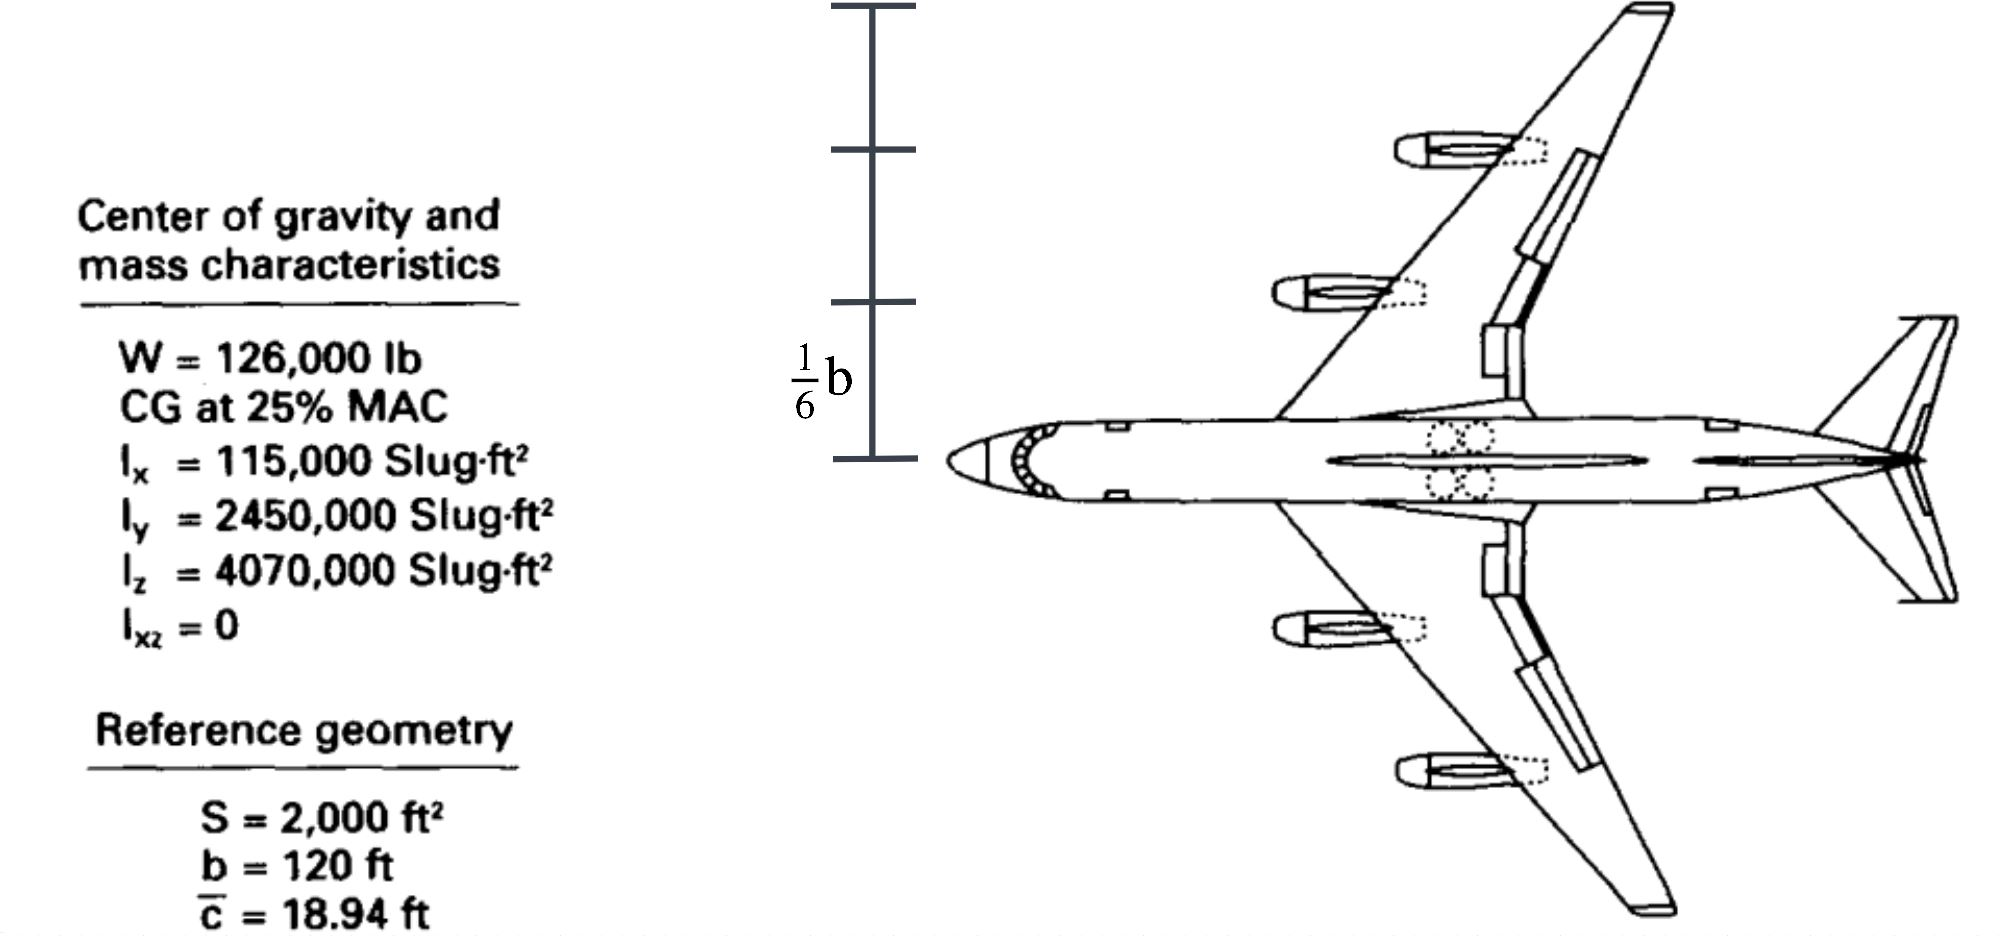
\includegraphics[width=0.85\textwidth]{figures/convair880.jpg}
\end{figure}
\begin{table}[htbp]
    \centering
    \caption{Lateral stability derivatives for the Convair 880 at sea level.}
    \begin{tabular}{cccccccccccc} % Adjust column alignment as needed
        \toprule
$C_{y_\beta}$ & $C_{l_\beta}$ & $C_{n_\beta}$ & $C_{l_p}$ & $C_{n_p}$ & $C_{l_r}$ & $C_{n_r}$ & $C_{l_{\delta_a}}$ & $C_{n_{\delta_a}}$ & $C_{y_{\delta_r}}$ & $C_{l_{\delta_r}}$ \\ % $C_{n_{\delta_r}}$ \\
-0.877 & -0.196 & 0.139 & -0.381 & -0.049 & 0.198 & -0.185 & -0.038 & 0.017 & 0.216 & 0.0226 \\ % & -0.096 \\ 
    \bottomrule
    \end{tabular}
\end{table}

\begin{enumerate}[label=\alph*)]
    \item If the aircraft operates with $C_L = 0.68$ and $C_D = 0.08$ what is minimum thrust that this aircraft must apply to remain in trim assuming that thrust is directly opposed to drag.
    
    \item Consider the case where the leftmost engine suddenly becomes non-responsive. The pilot wants to reduce the moment induced by the resulting asymmetry; however, the maximum thrust a single engine can contribute is $6000 \text{lb}_f$. What is the minimum yawing moment, $\Delta N_\text{thrust}$, that can be achieved by adjusting the individual throttles while maintaining the same total thrust? 

    \item Use a linear approximation to estimate the rudder power ($C_{n_{\delta_r}}$) needed so that flight with no sideslip can be maintained with an absolute rudder deflection of $3^\circ$ in this one-engine-out case.

    \item Use a linear approximation to estimate the aileron deflection and sideslip angle \textbf{in degrees} that would be needed to attain a steady flight condition in this one-engine-out case without any rudder deflection.
    
    % \item Using a linear approximation, estimate the surface area of the vertical stabilizer required so that a sideslip angle of $|\beta| \leq 10^\circ$ can be maintained with $|\delta_r| \leq 5^\circ$ and $|\delta_a| \leq 30^\circ$ in this one-engine-out condition. Assume that the listed derivatives are independent of the size of the tail.

    % \item Now the pilot want to enter the plane into a steady sideslip translation with an angle $\beta = 10^\circ$. What must the aileron and rudder deflections be to maintain this condition?

    % \item What must the surface area of the tail be in order to counteract the yawing moment?

    
\end{enumerate}
\end{question}
